% !TeX TS-program = xelatex


\documentclass[aspectratio=169]{beamer}

\usepackage{ctex}
\usepackage{fontspec}
\usepackage{tcolorbox}
\usepackage{metalogo}
\usepackage{tasks}
\usepackage{etoolbox}
\usepackage{expl3}
\usepackage{unicode-math}
\usepackage{minted}
\usepackage{xparse}
\usepackage{tikz}

\tcbuselibrary{minted,listings,xparse}

\usefonttheme{professionalfonts}
\usefonttheme{serif}

\setmonofont{IBMPlexMono-Regular}[
    Path=../fonts/,
    Extension=.ttf,
    BoldFont=IBMPlexMono-Bold,
    ItalicFont=IBMPlexMono-Italic,
    BoldItalicFont=IBMPlexMono-BoldItalic
]

\setmainfont{Roboto-Regular}[
    Path=../fonts/,
    Extension=.ttf,
    BoldFont=Roboto-Bold,
    ItalicFont=Roboto-Italic,
    BoldItalicFont=Roboto-BoldItalic
]

\setCJKmonofont{NotoSerifSC-Regular}[
    Path=../fonts/,
    Extension=.otf,
    BoldFont=NotoSerifSC-Bold,
    ItalicFont=NotoSerifSC-Regular
]

\setCJKmainfont{NotoSansSC-Regular}[
    Path=../fonts/,
    Extension=.otf,
    BoldFont=NotoSansSC-Bold
]

\setmathfont{TeX Gyre Termes Math}

\usetheme{AnnArbor}
\usecolortheme{beaver}
\setbeamertemplate{navigation symbols}{}

\author[项子越]{项子越\\ {\scriptsize\ttfamily ziyue.alan.xiang@gmail.com}}
\institute[]{\url{https://github.com/xziyue/latex3-chinese-video}}


% use custom lexer in minted
\newcommand{\pyltlexer}{../tex_lexer.py:Tex3Lexer -x}

\newcommand{\codefontsize}{\fontsize{7}{9}}

\newtcblisting{texcode}{
    listing only,
    listing engine=minted,
    minted options={
        fontsize=\codefontsize,
        linenos,
        autogobble,
        breaklines,
        numbersep=2mm,
        obeytabs,
        tabsize=2
    },
    minted language=\pyltlexer,
    top=0pt,
    bottom=0pt,
    left=4mm,
    colback=white,
    boxrule=1pt
}

\newtcblisting{texcode*}{
    listing engine=minted,
    minted options={
        fontsize=\codefontsize,
        linenos,
        autogobble,
        breaklines,
        numbersep=2mm,
        obeytabs,
        tabsize=2
    },
    minted language=\pyltlexer,
    top=0pt,
    bottom=0pt,
    left=4mm,
    colback=white,
    boxrule=1pt
}

%\newtcblisting{texcode**}{
%    listing engine=minted,
%    minted options={
%        fontsize=\codefontsize,
%        linenos,
%        autogobble,
%        breaklines,
%        numbersep=2mm,
%        obeytabs,
%        tabsize=2
%    },
%    minted language=\pyltlexer,
%    top=0pt,
%    bottom=0pt,
%    left=4mm,
%    colback=white,
%    boxrule=1pt,
%    listing side text
%}



\DeclareTCBListing{texcode**}{!o}{
    listing engine=minted,
    minted options={
        fontsize=\codefontsize,
        linenos,
        autogobble,
        breaklines,
        numbersep=2mm,
        obeytabs,
        tabsize=2
    },
    minted language=\pyltlexer,
    top=0pt,
    bottom=0pt,
    left=4mm,
    colback=white,
    boxrule=1pt,
    listing side text,
    IfValueTF={#1}{
        righthand width=\dimexpr #1\linewidth \relax
    }{}
}


\newtcblisting{progcode}[1]{
    listing only,
    listing engine=minted,
    minted options={
        fontsize=\codefontsize,
        linenos,
        autogobble,
        breaklines,
        numbersep=2mm,
        obeytabs,
        tabsize=2
    },
    minted language=#1,
    top=0pt,
    bottom=0pt,
    left=4mm,
    colback=white,
    boxrule=1pt
}

\renewcommand{\theFancyVerbLine}{\ttfamily \textcolor[rgb]{0.2,0.2.,0.2}{\fontsize{5}{7} \oldstylenums{\arabic{FancyVerbLine}}}}

\newmintinline[texinl]{\pyltlexer}{fontsize=\small}
\newmintinline[textinl]{text}{fontsize=\small}




\title{\LaTeX3教程二:变量,函数及基本程序结构}
\date{2021年3月22日}

\begin{document}

\maketitle

\newcommand{\dhrule}{%

\begin{tikzpicture}%
\draw[dashed, gray, ultra thick] (0,0)--(\linewidth, 0);
\end{tikzpicture}}

\newcommand{\lthint}{
{\scriptsize
\begin{itemize}
\item \texttt{tl}:凭据表
\item \texttt{str}:字符串
\item \texttt{int}:整型
\item \texttt{fp}:浮点数
\item \texttt{seq}:队列
\item \texttt{dim}:尺度/长度
\item \texttt{bool}:布尔型
\end{itemize}
\dhrule
\begin{itemize}
\item \texttt{N}:接收一个命令,传递命令本身。
\item \texttt{n}:接收一个凭据表。
\end{itemize}
}
}

\section{概括}

\begin{frame}
\begin{itemize}
\item 变量的声明和使用
\item 函数的声明和使用
\item 循环语句
\item 条件语句
\end{itemize}
\end{frame}

\section{变量}

\begin{frame}[fragile]

\begin{columns}
\begin{column}{0.5\linewidth}
声明变量:使用\textinl|new|结尾的函数
\begin{itemize}
\item \texinl|\bool_new:N|
\item \texinl|\int_new:N|
\item \texinl|\seq_new:N|
\item \texinl|\dim_new:N|
\item \texinl|\fp_new:N|
\end{itemize}
\end{column}
\begin{column}{0.5\linewidth}
\lthint
\end{column}
\end{columns}

\end{frame}



\begin{frame}[fragile]


\begin{columns}
\begin{column}{0.5\linewidth}
设置变量:使用\textinl|set|结尾的函数
\begin{itemize}
\item \texinl|\int_set:Nn|
\item \texinl|\dim_set:Nn|
\item \texinl|\fp_set:Nn|
\item \texinl|\bool_set_true:N|
\item \texinl|\bool_set_false:N|
\end{itemize}
\end{column}
\begin{column}{0.5\linewidth}
\lthint
\end{column}
\end{columns}

\end{frame}


\begin{frame}[fragile]

\begin{columns}
\begin{column}{0.5\linewidth}
使用变量:使用\textinl|use|结尾的函数
\begin{itemize}
\item \texinl|\int_use:N|
\item \texinl|\dim_use:N|
\item \texinl|\fp_use:N|
\item \texinl|\tl_use:N|
\item \texinl|\str_use:N|
\end{itemize}
\end{column}
\begin{column}{0.5\linewidth}
\lthint
\end{column}
\end{columns}

\end{frame}

\section{函数}

\begin{frame}[fragile]{声明函数}
使用\texinl|\cs_set:Npn|来声明函数。
\begin{texcode*}
\ExplSyntaxOn
\cs_set:Npn \my_function:n #1 {
    你输入了:#1
}
\par\my_function:n {一}
\par\my_function:n {二}
\ExplSyntaxOff
\end{texcode*}
\end{frame}

\begin{frame}{查阅函数文档}

获取\LaTeX3文档
\begin{itemize}
\item 搜索“CTAN l3kernel”
\item 点击“The LATEX3 interfaces”
\end{itemize}

{
\scriptsize
链接:\url{http://mirrors.ctan.org/macros/latex/contrib/l3kernel/interface3.pdf}
}

\begin{itemize}
\item 每一个章节对应一个\LaTeX3库
\item 每一个章节内的二级章节对应一系列功能类似的函数
\end{itemize}

\end{frame}


\begin{frame}{\LaTeX3文档中的函数条目}
\begin{figure}
\centering
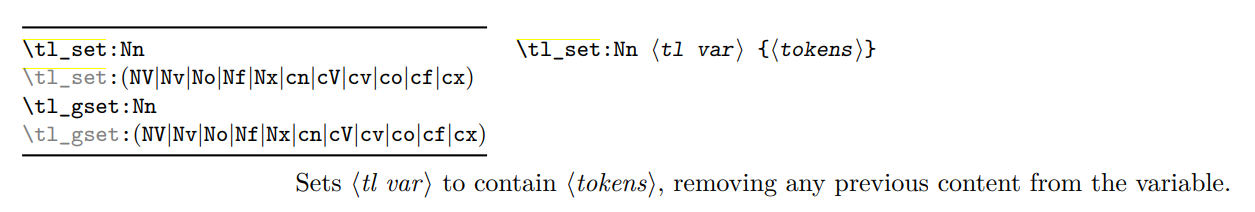
\includegraphics[width=0.95\linewidth]{l3_doc_func}
\end{figure}

\end{frame}


\begin{frame}{\LaTeX3文档中预定义的变量(scratch variables)}
\begin{figure}
\centering
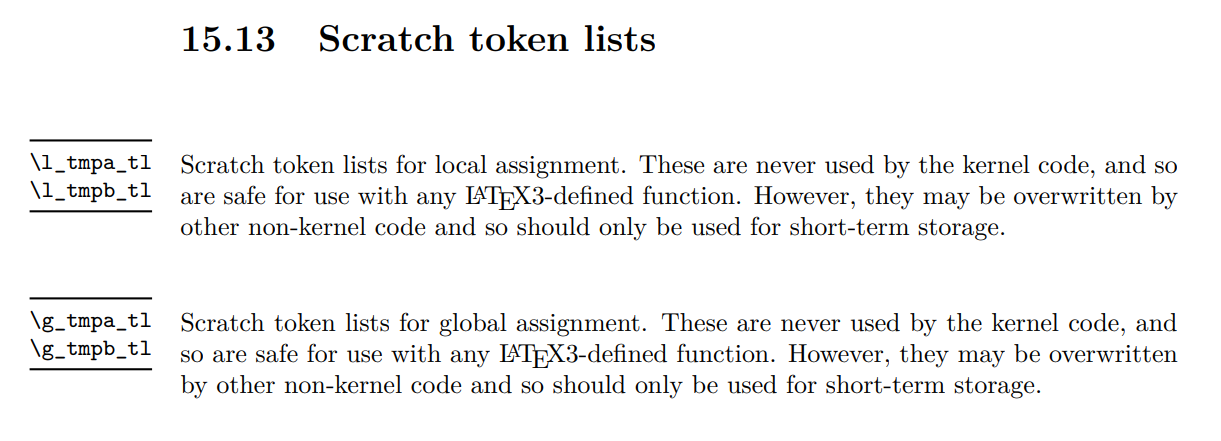
\includegraphics[width=0.85\linewidth]{l3_doc_scratch_var}
\end{figure}
\begin{itemize}
\item 在文档比较庞大时,尽量避免使用这些变量以防止冲突
\end{itemize}
\end{frame}

\begin{frame}[fragile]{案例:加法}
\begin{texcode*}
\ExplSyntaxOn
\int_new:N \l_my_tmpa_int
\int_new:N \l_my_tmpb_int
\int_set:Nn \l_my_tmpa_int {200}
\int_set:Nn \l_my_tmpb_int {10}
\int_eval:n {\l_my_tmpa_int + \l_my_tmpb_int}
\ExplSyntaxOff
\end{texcode*}
\end{frame}

\section{循环语句}

\begin{frame}[fragile]{基于整数的循环}
\begin{texcode**}
\ExplSyntaxOn
\int_step_inline:nn {20} {
    #1,~
}
\ExplSyntaxOff
\end{texcode**}
\end{frame}

\begin{frame}[fragile]{基于整数的循环}
改变起始数值
\begin{texcode**}
\ExplSyntaxOn
\int_step_inline:nnn {10} {20} {
    #1,~
}
\ExplSyntaxOff
\end{texcode**}
\end{frame}

\begin{frame}[fragile]{基于整数的循环}
将循环变量保存在凭据表中
\begin{texcode**}
\ExplSyntaxOn
\int_step_variable:nNn {20} \l_tmpa_tl {
    \tl_use:N \l_tmpa_tl,~
}
\ExplSyntaxOff
\end{texcode**}
\end{frame}

\begin{frame}[fragile]{基于整数的循环}
二重循环
\begin{texcode**}
\ExplSyntaxOn
\int_step_inline:nn {5} {
    \int_step_inline:nn {5} {
        (#1,##1), ~
    }
}
\ExplSyntaxOff
\end{texcode**}
\end{frame}

\begin{frame}[fragile]{案例:$1+2+\ldots+100=?$}
\begin{texcode*}
\ExplSyntaxOn
\int_set:Nn \l_tmpa_int {0}
\int_step_inline:nn {100} {
    \int_add:Nn \l_tmpa_int {#1}
}
\int_use:N \l_tmpa_int
\ExplSyntaxOff
\end{texcode*}
\end{frame}

\begin{frame}[fragile]{案例:圆上的点}
圆的参数方程: 
{\scriptsize $\begin{cases}
x = r\cos\theta\\
y = r\sin\theta
\end{cases}$}
\begin{texcode**}
\ExplSyntaxOn
\begin{tikzpicture}
\int_step_inline:nnn {0} {17} {
    \fp_set:Nn \l_tmpa_fp {20 * (#1) * \c_one_degree_fp}
    \node[minimum~width=1.5mm, fill=blue, 
        draw=none, circle, inner~sep=0pt] at 
    (\fp_eval:n {cos(\l_tmpa_fp)}, 
     \fp_eval:n {sin(\l_tmpa_fp)}) {};
}
\end{tikzpicture}
\ExplSyntaxOff
\end{texcode**}

\end{frame}


\section{条件语句}

\begin{frame}[fragile]{整数判断}
\begin{texcode*}
\ExplSyntaxOn
\cs_set:Npn \my_if_less_than_two:n #1 {
    \int_compare:nNnTF {#1} < {2} {
        \zhnumber{#1} 小于二
    } {
        \zhnumber{#1} 大于等于二
    }
}
\par\my_if_less_than_two:n {1}
\par\my_if_less_than_two:n {2}
\par\my_if_less_than_two:n {3}
\ExplSyntaxOff
\end{texcode*}
\end{frame}

\begin{frame}[fragile]{整数判断}
\begin{texcode*}
\ExplSyntaxOn
\cs_set:Npn \my_if_less_than_two:n #1 {
    \int_compare:nTF {#1 <= 2} {
        \zhnumber{#1} 小于等于二
    } {
        \zhnumber{#1} 大于二
    }
}
\par\my_if_less_than_two:n {1}
\par\my_if_less_than_two:n {2}
\par\my_if_less_than_two:n {3}
\ExplSyntaxOff
\end{texcode*}
\end{frame}

\begin{frame}[fragile]{布尔判断}
\begin{itemize}
\item 使用\texinl|\bool_if:nTF|可以进行布尔判断;其表达式参数支持\textinl|&&|, \textinl!||!, \textinl|()|等逻辑运算符
\item 一般的判断语句还有\textinl|_p|变体,例如\texinl|\int_compare_p:n|, \texinl|\bool_if_p:n|等。这些函数不是根据判断结果执行分支,而是直接返回判断结果为真或为假
\item 这些“判别式”(predicate)可以帮助我们构建复杂的逻辑语句
\end{itemize}
\end{frame}

\begin{frame}[fragile]{案例:偶数判断}
\begin{texcode*}
\ExplSyntaxOn
\cs_gset:Npn \my_if_even_p:n #1 {
    \int_compare_p:nNn {\int_mod:nn {#1}{2}} = {0}
}
\cs_set:Npn \my_even_check:n #1 {
    \bool_if:nTF { \my_if_even_p:n {#1}} {
        \zhnumber{#1}是偶数
    } {
        \zhnumber{#1}是奇数
    }
}
\par \my_even_check:n{1}
\par \my_even_check:n{2}
\par \my_even_check:n{3}
\ExplSyntaxOn
\end{texcode*}
\end{frame}


\begin{frame}[fragile]{案例:双偶数判断}
\begin{texcode*}
\ExplSyntaxOn
\cs_set:Npn \my_double_even_check:nn #1#2 {
    \bool_if:nTF { \my_if_even_p:n {#1} && \my_if_even_p:n {#2}} {
        \zhnumber{#1}和\zhnumber{#2}都是偶数
    } {
        \zhnumber{#1}和\zhnumber{#2}不都是偶数
    }
}
\par \my_double_even_check:nn {1} {3}
\par \my_double_even_check:nn {1} {2}
\par \my_double_even_check:nn {2} {4}
\ExplSyntaxOn
\end{texcode*}
\end{frame}


\section{循环与判断}

\begin{frame}[fragile]{条件循环语句}
诸如\texinl|\int_do_while:nNnn|, \texinl|\bool_do_while:nn|等语句每一次循环就进行一次判断,直到判断为假。
\begin{texcode*}
\ExplSyntaxOn
\int_set:Nn \l_tmpa_int {1}
\int_set:Nn \l_tmpb_int {0}
\int_do_while:nNnn {\l_tmpa_int} < {101} {
    \int_add:Nn \l_tmpb_int {\l_tmpa_int}
    \int_incr:N \l_tmpa_int
}
\int_use:N \l_tmpb_int
\ExplSyntaxOff
\end{texcode*}
\end{frame}

\begin{frame}[fragile]{条件循环语句}
诸如\texinl|\int_do_until:nNnn|, \texinl|\bool_do_until:nn|等语句每一次循环就进行一次判断,直到判断为真。
\begin{texcode*}
\ExplSyntaxOn
\int_set:Nn \l_tmpa_int {1}
\int_set:Nn \l_tmpb_int {0}
\int_do_until:nNnn {\l_tmpa_int} > {100} {
    \int_add:Nn \l_tmpb_int {\l_tmpa_int}
    \int_incr:N \l_tmpa_int
}
\int_use:N \l_tmpb_int
\ExplSyntaxOff
\end{texcode*}
\end{frame}

\end{document}